\documentclass[12pt, twoside]{article}
\usepackage[letterpaper, margin=1in, headsep=0.5in]{geometry}
\usepackage[english]{babel}
\usepackage[utf8]{inputenc}
\usepackage{amsmath}
\usepackage{amsfonts}
\usepackage{amssymb}
\usepackage{tikz}
\usetikzlibrary{quotes, angles}
\usepackage{graphicx}
%\usepackage{pgfplots}
%\pgfplotsset{width=10cm,compat=1.9}
%\usepgfplotslibrary{statistics}
%\usepackage{pgfplotstable}
%\usepackage{tkz-fct}
%\usepackage{venndiagram}

\usepackage{fancyhdr}
\pagestyle{fancy}
\fancyhf{}
\renewcommand{\headrulewidth}{0pt} % disable the underline of the header

\fancyhead[RE]{\thepage}
\fancyhead[RO]{\thepage \\ Name: \hspace{3cm}}
\fancyhead[L]{BECA / Dr. Huson / Geometry 10th Grade\\* Unit 2: Midpoints and distance \\ 
25 September 2019}

\begin{document}
  \subsubsection*{2.7 Classwork: Modeling with a drawing and equation}
  \begin{enumerate}
    \subsubsection*{Do Not Solve! Make a drawing on the right, an equation to the left, and circle where it states what to find.}
    \vspace{0.5cm}

\item The point $Q$ is the midpoint of $\overline{PR}$, $PQ=12$, and $QR=x+3$. Find ${x}$.
\vspace{4cm}

\item Given $\overline{PQR}$, with $PQ=2x-5$, $QR=x+3$, and $PR=19$. Find ${x}$.
\vspace{4cm}

\item Given that $Q$ bisects $\overline{PR}$. $PQ=2x-5$, $QR=x+3$. Find ${PR}$.
\vspace{4cm}

\item The points $P$, $Q$, and $R$ are collinear, with $PQ=3x+14$, $QR=2x+2$, and $PR=6x+12$. Find ${PQ}$.
\vspace{4cm}

\newpage

\item Angles $P$ and $Q$ are supplementary. $m\angle P = x+57$ and $m\angle Q = 3x-11$. Find $m\angle Q$. \vspace{3.5cm} 

\item Given two complementary angles, $m\angle A = 5x+14$ and $m\angle B = 3x-9$. Find the measure of $\angle B$. \vspace{3.5cm} 

\item Given $\angle P \cong \angle Q$. $m\angle P = 3x+20$ and $m\angle Q = 2x-10$. Find $m\angle Q$. \vspace{3.5cm} 

\subsubsection*{For the following problem, calculate the length.}

\item Given $\overline{DEFG}$, $DE=3 \frac{3}{7}$, $EF=4 \frac{3}{14}$, and $FG= 2 \frac{5}{14}$. (diagram not to scale)\\ [0.25cm]
  Find ${DG}$.\\[.5in]
      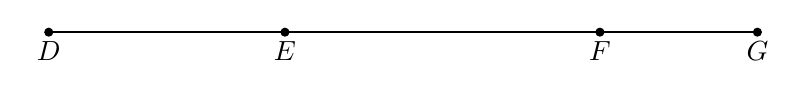
\begin{tikzpicture}
        \draw [-, thick] (0,0)--(9,0);
        \draw [fill] (0,0) circle [radius=0.05] node[below]{$D$};
        \draw [fill] (3,0) circle [radius=0.05] node[below]{$E$};
        \draw [fill] (7,0) circle [radius=0.05] node[below]{$F$};
        \draw [fill] (9,0) circle [radius=0.05] node[below]{$G$};
      \end{tikzpicture}
      \vspace{4cm}

\end{enumerate}
\end{document}
